\chapter{Fundamentals}
 In this chapter, we first review some fundamental properties of continuous dynamical systems that will be used heavily in later chapters. As we will see, these technical results are interesting in their own right. They can help in interpreting or cross-checking numerical results or physical models for self-consistency or accuracy.
\section{Existence and uniqueness of solutions}
Consider  
\begin{align}
\begin{dcases}
	\dot{x} = f(x,t); & x \in \mathbb{R}^{n} \\
	x(t_0) = x_0
\end{dcases}.
\end{align}
Does this initial value problem have a unique solution? We have the following theorems to help us answer that question.
\begin{theorem}[Peano]
	\label{thm:Peano}
	If $f\in C^0$ near $(x_0, t_0)$, then there exists a local solution $\varphi(t)$, i.e., 
\begin{align}
	\dot{\varphi}(t) = f(\varphi(t), t), \varphi(t_0) = x_0;\ \forall  t\in (t_0 - \epsilon, t_0 + \epsilon);\ 0<  \epsilon \ll 1.
\end{align}
\end{theorem}
\begin{ex}[Free falling mass]
	Consider a point mass of mass $m$ at position $x$. The acceleration due to gravity is denoted by $g$. Measuring the potential energy from the reference point $x=x_0$, we have that the total energy is conserved
	\begin{align}
		\frac{1}{2} m \dot{x}^2 = mg(x-x_0).
	\end{align}
This implies that
\begin{align}
	\begin{dcases}
		\dot{x} = \sqrt{2g(x-x_0)} \\
		x(0) = x_0
	\end{dcases}
\end{align}
on the set $P = \{ x \in \mathbb{R}:\ x \geq x_0\}$. Therefore we have that $f\in C^0$ in phase space, so by Peano's theorem (cf. Theorem \ref{thm:Peano}), there exists a local solution. A schematic diagram is shown in Fig. \ref{fig:chap1:1}. 
	\begin{figure}[H]
		\label{fig:chap1:1}
		\centering
		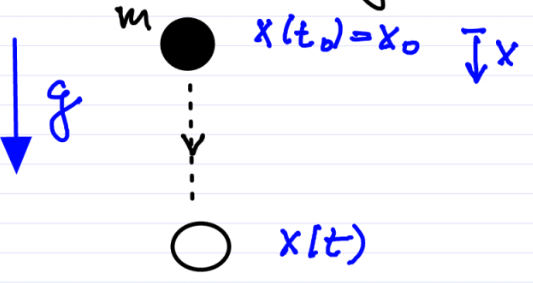
\includegraphics[width=0.4\textwidth]{figures/ch1/1freefall.png}
		\caption{Schematic diagram of the point mass in free fall.}
	\end{figure}
	The solution is actually $x(t) = x_0 + \frac{g}{2}(t-t_0)^2$, however $x(t) = x_0$ is also a solution to the IVP, therefore we do not have a unique solution. Physically there exists a solution, but this IVP was derived from a heuristic energy-principle, not from Newton's laws, which are not equivalent.
\end{ex}
\begin{definition}
A function $f$ is called locally Lipschitz around $x_0$ if there exists an open set $U_{x_0}$ and $L>0$ such that for all $x,y \in U_{x_0}$
\begin{align}
	\boxed{\left| f(y,t) - f(x,t)\right| \leq L |y - x|.}
\end{align}
\end{definition}

\begin{ex}[Lipschitz functions]
	Fig. \ref{fig:chap1:2} shows an example of a Lipschitz and a non-Lipschitz function around $x_0$.
	\begin{figure}[h]
		\label{fig:chap1:2}
		\centering
		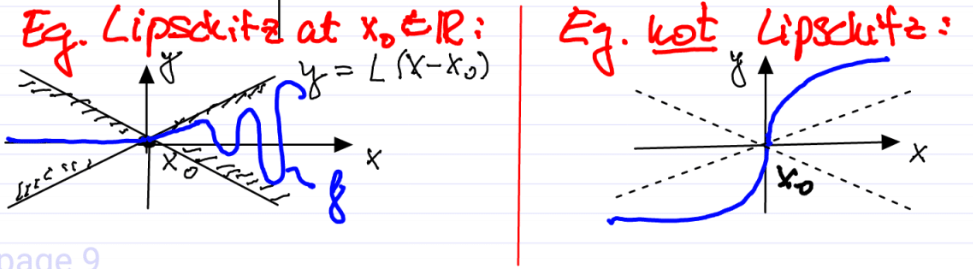
\includegraphics[width=0.8\textwidth]{figures/ch1/2lipschitz.png}
		\caption{Interpretation of the Lipschitz property.}
	\end{figure}
\end{ex}

\begin{theorem}[Picard]
	Assume 
	\begin{enumerate}
		\item  $f \in C^0$ in $t$ near $(t_0, x_0)$,
		\item $f$ is locally Lipschitz in $x$ near $(t_0, x_0)$.
	\end{enumerate}
	Then there exists a unique local solution to the IVP. The proof can be found in Arnold's book on ODEs.  	
\end{theorem}
\textbf{Note} the following relations. If $f$ is $C^1$ $\implies$ $f $ is Lipschitz $\implies $ $f$ is $C^0$. 
\begin{ex}[Free falling mass revisted]
	We check if $f$ is Lipschitz.
	\begin{align}
		\frac{| f(x) - f(x_0) |}{|x-x_0|} = \frac{\sqrt{2g}}{\sqrt{|x-x_0|}} \not< L | x - x_0|.
	\end{align}
Thus $f$ is not Lipschitz near $x_0$.	
\end{ex}

\section{Geometric consequences of uniqueness}
If the solution is unique, we have a few facts that can be derived from the geometric point of view.
\begin{itemize}
	\item[(i)] The trajectories of autonomous systems cannot intersect. Note that fixed points do not violate this. See Fig. \ref{fig:chap1:3} which shows the phase portrait of the pendulum. 
	\end{itemize}

		\begin{figure}[H]
			\centering
			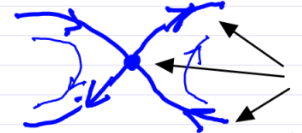
\includegraphics[width=0.3\textwidth]{figures/ch1/3pendulum_trajectories.png}
			\caption{The phase portrait of the pendulum. Trajectories do not intersect since each arrow is pointing at separate trajectories.}
			\label{fig:chap1:3}

		\end{figure}
\begin{itemize}
	\item[(ii)] For non-autonomous systems, intersections in phase space are possible: a trajectory may occupy the same point $x$ at different time instants (see the left panel of Fig. \ref{fig:chap1:4}). In this case we can extend the phase space in order to get an autonomous system where there cannot be any intersections.
			\begin{figure}[H]
			\centering
			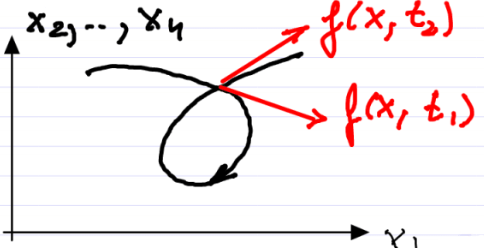
\includegraphics[width=0.4\textwidth]{figures/ch1/4intersecting_trajectories.png}
			\hspace{0.05\textwidth}
			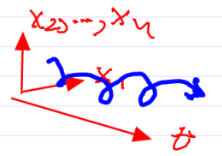
\includegraphics[width=0.3\textwidth]{figures/ch1/5extended_space.png}
			\caption{Left: Intersecting trajectories in phase space for a non-autonomous system. Right: The same trajectory in the extended phase space, without intersections.}
			\label{fig:chap1:4}

		\end{figure}
		
		\begin{align}
			X = 
			\begin{pmatrix}
				x \\ t
			\end{pmatrix},\
			F(X) = 
			\begin{pmatrix}
				f(x,t) \\ 1
			\end{pmatrix};\
			\dot{X} = F(X).
		\end{align}
\end{itemize}

\section{Local vs global existence}
\begin{ex}[Exploding solution]
	\begin{align}
		\begin{dcases}
			\dot{x} = x^2 \\
			x(t_0) = 1.
		\end{dcases}
	\end{align}
	Integrating yields the solution $x(t) = \frac{1}{1 - (t-t_0)}$. This solution blows up at $t_{\infty }=t_0 + 1$, therefore the solution is only local.	This is demonstrated in Fig. \ref{fig:chap1:5}.
\begin{figure}[H]
\centering	
\begin{tikzpicture}
	\begin{axis}
		[xmin=0, xmax=2.5, ymin=0.5, ymax=3, domain = 1:1.9, xlabel=$t$, ylabel=$x(t)$, xtick=\empty, ytick=\empty]
		\addplot[color=black] {1/(2-x)};
		\addplot[color=black, dashed] coordinates {(1.7,0.5) (1.7,3.1)} node[pos=0, above right] {$t_{\infty }$};
		\addplot[color=black, dashed] coordinates {(1,0.5) (1,1)} node[pos=0, above right] {$t_{0}$};
		\addplot[color=black, dashed] coordinates {(0,1) (1,1)} node[pos=0, above right] {$x_{0}$};
	\end{axis}
\end{tikzpicture}
\caption{Solution to the ODE $\dot{x}=x^2$ started from $x(t_0)=1$.}
\label{fig:chap1:5}
\end{figure}
\end{ex}
To address this problem of local solutions not being able to be continued into global solution, we have the following theorem.
\begin{theorem}[Continuation of solution]
	If a local solutions cannot be continued to a time $t=T$, then we must have
	\begin{align}
		\boxed{\lim_{t\to T} |x(t)|= \infty.}
	\end{align}
The proof can be found in Arnold's book on ODEs.
\end{theorem}

\begin{ex}[Coupled Pendulum System] Consider two pendulums of masses $m_1$ and $m_2$. They both have  length $l$. The angles of these pendula are denoted by $\varphi_1$ and $\varphi_2$. Let us assume that they are coupled by a nonlinear spring, which can be described by a potential $V(\varphi_1, \varphi_2)$. This setup is illustrated in Fig. \ref{fig:chap1:6}. 
	We set $x_1 = \varphi_1,\ x_2 = \dot{\varphi_1},\ x_3 = \varphi_2,\ x_4=\dot{\varphi_2} $ and get the following equation of motion
\begin{align}
	\begin{dcases}
		\dot{x}_1 = x_2 \\ \dot{x}_2 = \ldots \\ \dot{x}_3 = x_4 \\ \dot{x}_4 = \ldots
	\end{dcases}
\end{align}
The RHS is smooth, therefore there exists a unique local solution to any IVP.
\begin{figure}[h]
	\centering
	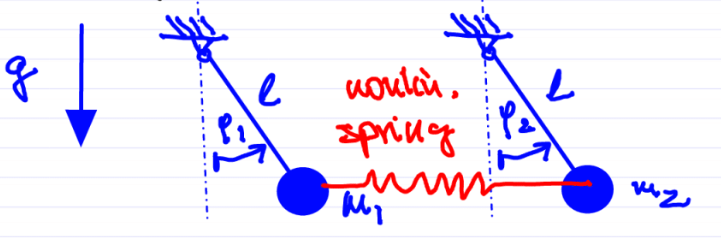
\includegraphics[width=0.6\textwidth]{figures/ch1/6coupled_pendulum.png}
	\caption{Physical setup of the coupled pendulum with a nonlinear spring.}
	\label{fig:chap1:6}
\end{figure}
The phase space is given by 
\begin{align}
	P = \{x:\ x_1 \in S^1,\ x_2 \in \mathbb{R},\ x_3 \in S^1,\ x_4 \in \mathbb{R} \} = S^1 \times \mathbb{R}\times S^1 \times \mathbb{R}.
\end{align}
Where $S^1$ is the 1 dimensional sphere (i.e. a circle). With this space we know that $|x_1|$ and $|x_3|$ are bounded. Due to energy being conserved we have
\begin{align}
	E &= T+V = \frac{1}{2}m_1 l_1 x_2^2 + \frac{1}{2}m_2 l_2 x_4^2 + \underbrace{V(x_1, x_3)}_{\geq 0}\\
	E &= E_0 =  \textrm{constant} \geq 0.
\end{align}
Hence $|x_2|$ and $|x_4|$ are also bounded, therefore all solutions exist globally.
\end{ex}
\begin{definition}
	A linear system is one such that for $x\in \mathbb{R}^{n},\ A(t) \in \mathbb{R}^{n\times n}$ and $A\in C^0$ 
	\begin{align}
		\boxed{\dot{x} = A(t) x.}
	\end{align}
\end{definition}

\begin{remark}[]
	Note that  $S = \frac{1}{2}(A + A^T)$ is symmetric (i.e. $S = S^T)$ and $\Omega = \frac{1}{2}(A - A^T)$ is skew symmetric (i.e. $\Omega = -\Omega^T$). Furthermore the eigenvalues of $S$, $\lambda_i$, are all real and their respective eigenvectors, $e_i$, are orthogonal.
\end{remark}

\begin{ex}[Global existence in linear systems]
\begin{align}
	\langle x, \dot{x} \rangle &= \frac{1}{2} \frac{d}{dt} |x(t)|^2 = \langle x, A(t) x\rangle = \langle x, (S(t) + \Omega(t) ) x \rangle \\
				   &= \langle x, S(t) x \rangle + \underbrace{\langle x, \Omega(t) x \rangle}_{=0} \stackrel{(*)}{=} 
				   \sum_{i=1}^{n} \lambda_i(t) x_i^2 \\
				   &\leq \lambda_{ \textrm{max} }(t) \sum_{i=1}^{n} x_i^2 = \lambda _{ \textrm{max} }(t) | x(t)|^2.
\end{align}
Where in $(*)$ we used that $x = \sum_{i=1}^{n} x_i e_i $ with $|e_i|=1$ and $e_i \perp e_j$ for all $i \neq j$. Thus we get
\begin{align}
	\frac{\frac{1}{2}\frac{d}{dt}|x(t)|^2}{|x(t)|^2} \leq \lambda_{ \textrm{max} }(t) 
	\implies \int_{t_0}^{t} \log \left( \frac{|x(s)|^2}{|x(t_0)|^2} \right) ds \leq \lambda _{ \textrm{max} }(s) ds.
\end{align}
By exponentiating both sides, we obtain
\begin{align}
\boxed{ |x(t)| \leq |x(t_0) | \exp\left(\int_{t_0}^{t} \lambda_{ \textrm{max} }(s)ds\right).}
\end{align}
Therefore, by the continuation theorem, global solutions exist as long as $\int_{t_0}^{t} \lambda_{ \textrm{max} }(s) ds < \infty $.
\end{ex}

\section{Dependence on initial conditions}
Given the IVP
\begin{align}
	\begin{dcases}
	\dot{x} = f(x,t) \\ x(t_0) = x_0.
	\end{dcases}
\end{align}
With $x \in \mathbb{R}^{n}$ and $f\in C^r$ for some $r\geq 1$, we have the solution $x(t; t_0, x_0)$.

\textbf{Question} How does the solution depend on initial data?
But first, why do we care about this? Because we expect solution that are robust with respect to errors and uncertainties in the initial data.
\begin{theorem}[]
	If $f \in C^r$ for $r\geq 1$ then $x(t; t_0, x_0)$ is $C^r$ in $(t_0, x_0)$. Proof in Arnold's ODE.
\end{theorem}

The geometric meaning of this is that for $U \subset P \subset \mathbb{R}^{n}$ we have that $F_{t_0}^{t}(U)$ is a smooth deformation of $U$ (see Fig. \ref{fig:chap1:7}).
\begin{figure}[h]
	\centering
	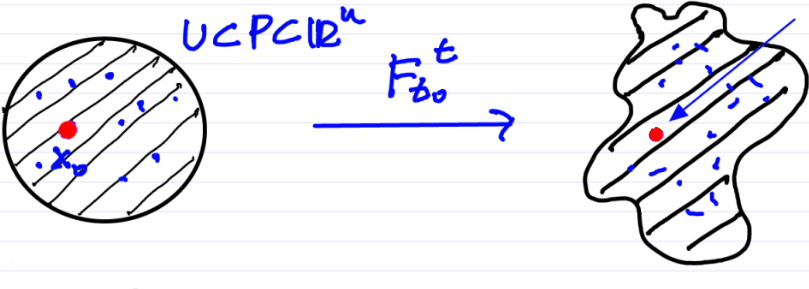
\includegraphics[width=0.7\textwidth]{figures/ch1/7smooth_transform.png}
	\caption{The smooth transformation of $U$. The red point on the right is $F _{t_0}^t(x_0)$, i.e., the image of $x_0$ under the evolution operator.}
	\label{fig:chap1:7}
\end{figure}
It turns out $\left(F_{t_0}^{t}\right)^{-1} = F_{t}^{t_0}$ is also $C^r$, hence we have that $F_{t_0}^{t}$ is a diffeomorphism. 

Now, how can we compute the Jacobian of the flow map $\frac{\partial x(t; t_0, x_0)}{ \partial x_0} = DF _{t_0}^{t}(x_0)$? We start from the IVP and take the gradient (with respect to $x_0$) of both sides. On the left hand side we can exchange order of the time derivative and the gradient and on the right hand side we use the chain rule. We end up with the equation
\begin{align}
	\frac{d}{dt}\frac{\partial x}{\partial x_0} = D_x f(x(t; t_0, x_0), t) \frac{\partial x}{\partial x_0}.
\end{align}
This means, that the flow map gradient satisfies the IVP
\begin{align}
	\frac{d}{dt}\left[ DF_{t_0}^{t}(x_0)\right] &= D_{x}f(F_{t_0}^{t}(x_0), t) DF_{t_0}^{t}(x_0) \\
	DF_{t_0}^{t_0}(x_0) &= I.
\end{align}
This is called the equation of variations, which is a linear, non-autonomous ODE for the matrix $M = DF _{t_0}^{t}(x_0)$
\begin{align}
	\begin{dcases}
		\dot{M} = D_x f(x(t; t_0, x_0)) M \\ M(t_0) = I.
	\end{dcases}
\end{align}
